
\documentclass{article}
\usepackage[english]{babel}
\usepackage[T1]{fontenc}

\usepackage[usenames, dvipsnames]{color}
\usepackage{uarial}
\renewcommand{\familydefault}{\sfdefault}
\usepackage{blindtext}
\usepackage{Sweave}
\begin{document}


\Sconcordance{concordance:pdfCreator.tex:pdfCreator.Rnw:%
1 9 1 1 0 4 1 1 21 9 1 1 3 1 5 25 1}




\section*{\textcolor{Fuchsia}{Smoking Prevalence in Adults*}}

Now lets try and dothisWe could maybe use this for RBCO. RSweave docs in RStudio are like RMarkdown but just for latex and and pdf creation. It has full latex support and nice to work with. We can put plots in with no problem and build the layout around that.
I'm writing something here to test
several features.
\break
\break

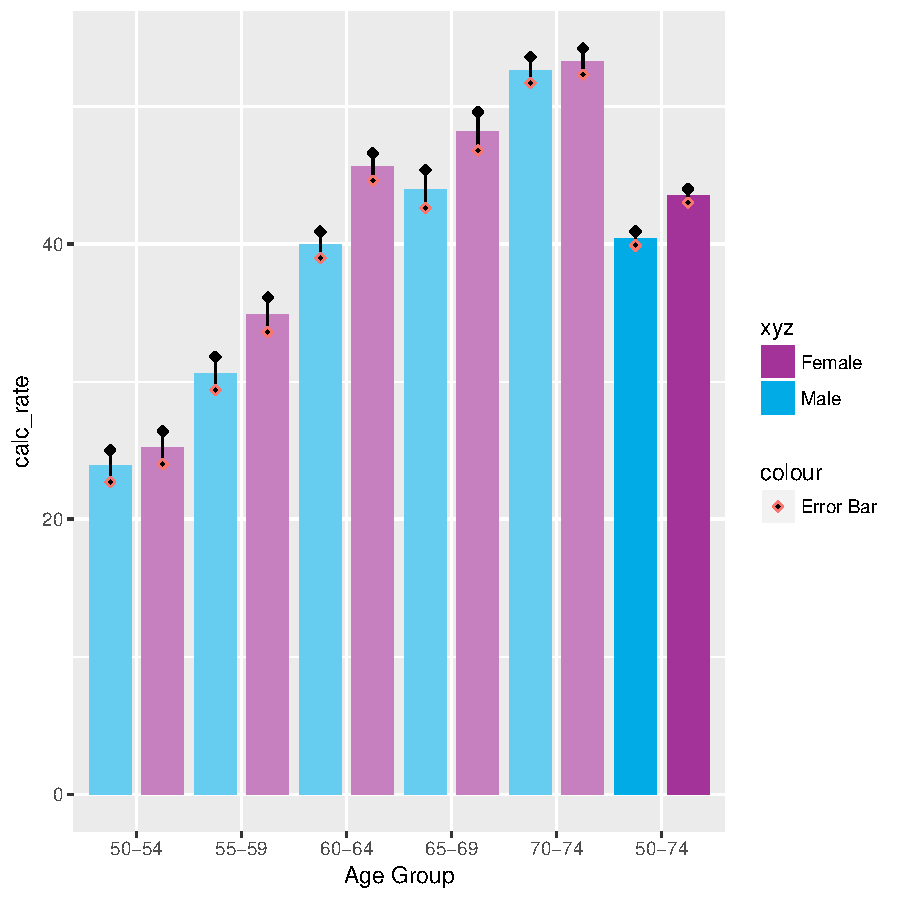
\includegraphics{pdfCreator-002}


\def\dashfill{\cleaders\hbox{-}\hfill}
\hbox to \hsize{\dashfill\hfil}
\bye
* Persons aged over 16 \newline
Notes: 

\begin{enumerate}
  \item All the typesettign stuff, everything from page number positioning to footnotes can be done in latex and the workflow for using it in an RSweave doc (the way RStudio does this) is really nice
  \item Is very easy to make tiny typesetting changes - Latex was designed for preducing camera ready papers. 
  \item This is a nice workflow for doing any acadmic stuff, so nice to push it into RBCO publishing
   
\end{enumerate}

\break
asdf
\break


\section*{Another title}

We could maybe use this for RBCO. RSweave docs in RStudio are like RMarkdown but just for latex and and pdf creation. It has full latex support and nice to work with. We can put plots in with no problem and build the layout around that.


\end{document}
